\documentclass{article}
\usepackage[utf8]{inputenc}
\usepackage{graphicx}
\begin{document}

\section{Bisection algorithm for simplical meshes}
\label{sec:title}

\begin{itemize}
	\item Serial algorithm
	\item Longest edge splitting with propagation front
	% \item Local refinement propagation so that the levels of refinement of the one-ring
	% neighbors it differs at most one.
	\item For 2D meshes with triangles isosceles the number of congruence classes is 1. 
	\item The algorithm works directly for 3D and 4D.
\end{itemize}

\begin{figure}[htbp]
	\centering
	\parbox{0.5\linewidth}{
	
\includegraphics[width=0.32\linewidth]{figures/mesh_2_bisect_1} \hfill
	
\includegraphics[width=0.32\linewidth]{figures/mesh_2_bisect_2} \hfill
	
\includegraphics[width=0.32\linewidth]{figures/mesh_2_bisect_3} \par
	
\includegraphics[width=0.32\linewidth]{figures/mesh_2_bisect_4} \hfill
	
\includegraphics[width=0.32\linewidth]{figures/mesh_2_bisect_5} \hfill
	
\includegraphics[width=0.32\linewidth]{figures/mesh_2_bisect_6} \par
	
\includegraphics[width=0.32\linewidth]{figures/mesh_2_bisect_7} \hfill
	
\includegraphics[width=0.32\linewidth]{figures/mesh_2_bisect_8} \hfill
	
\includegraphics[width=0.32\linewidth]{figures/mesh_2_bisect_9} \par
	}
	\caption{Steps of the bisection algorithm.}
	\label{fig:two_dim}
\end{figure}

\begin{figure}[htbp]
	\centering
	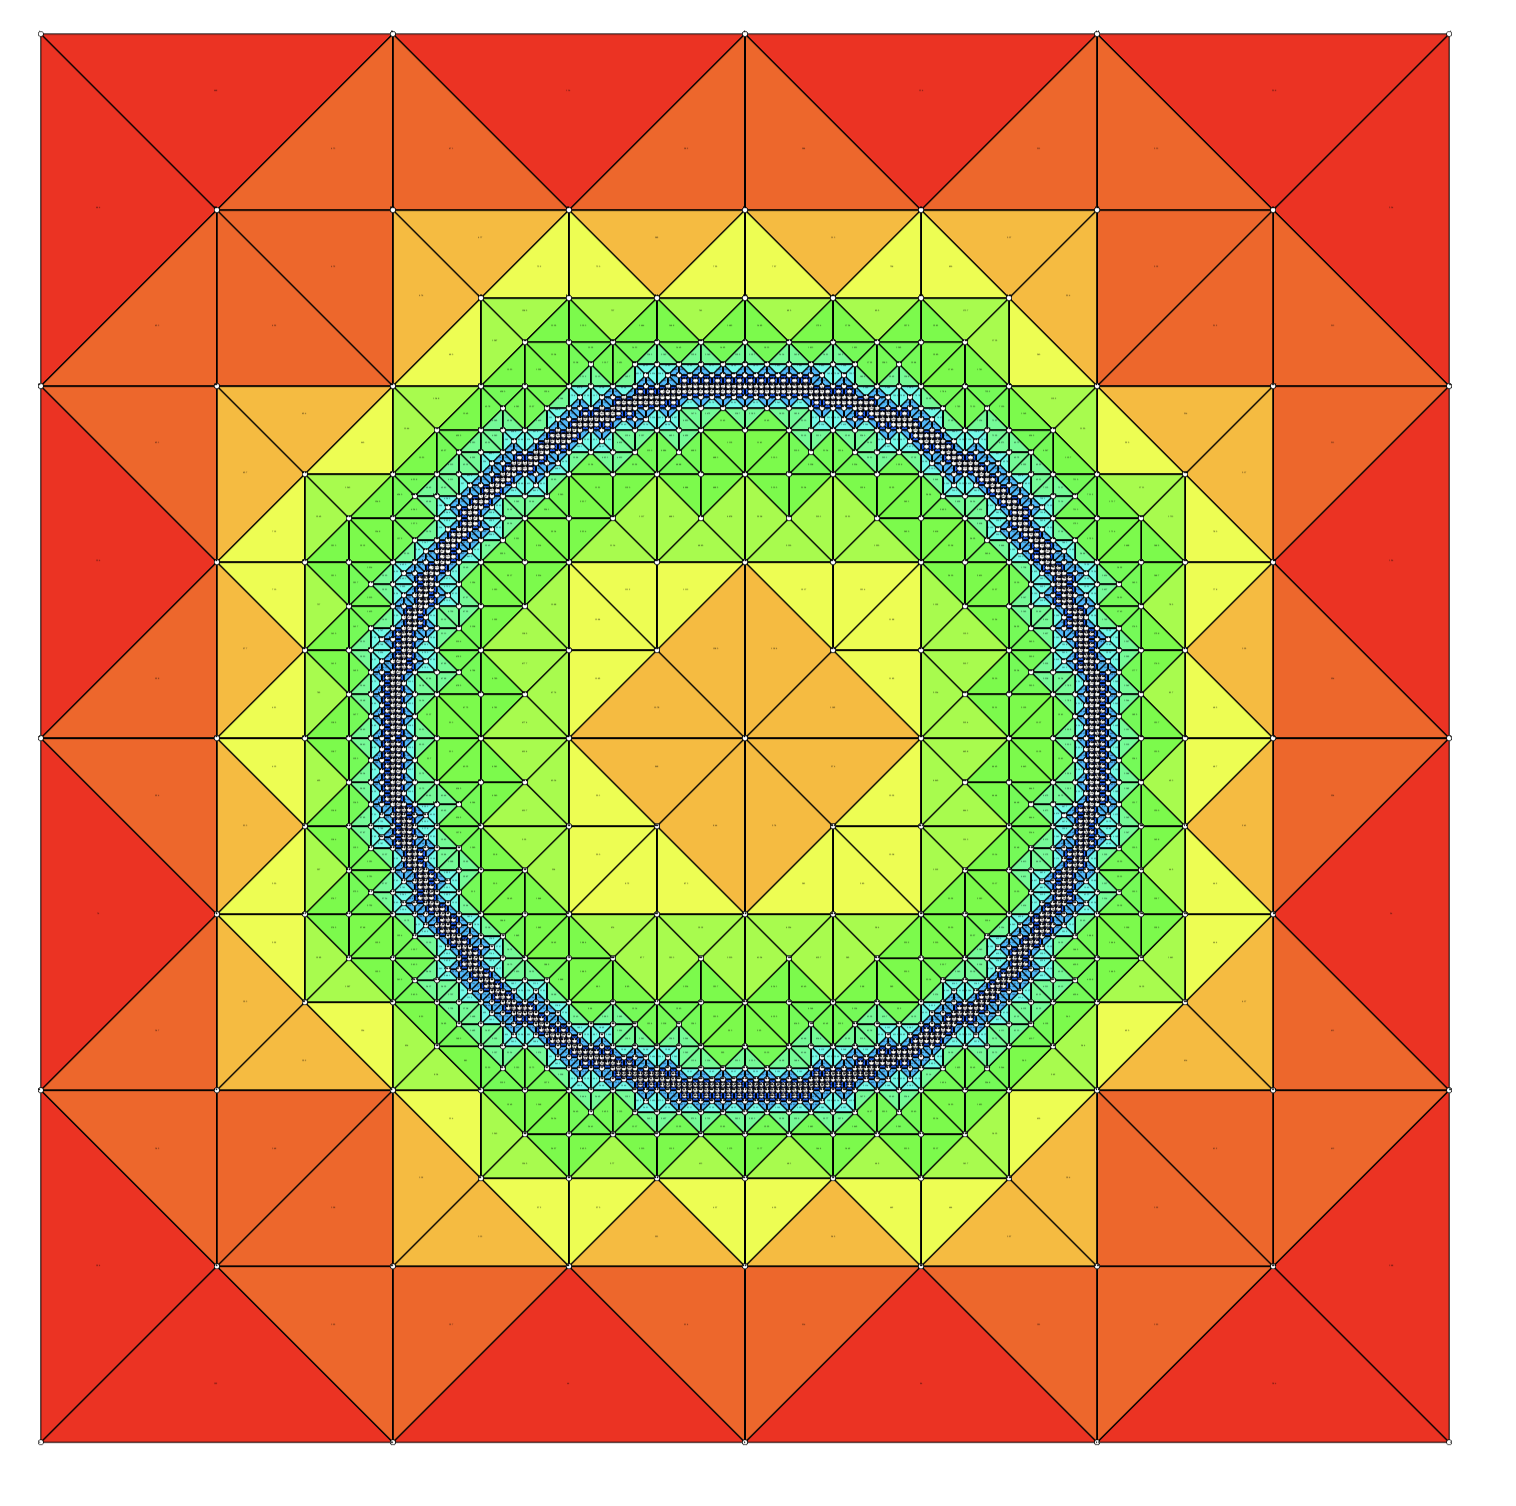
\includegraphics[width=0.40\linewidth]{figures/2d_sphere} \hfill
	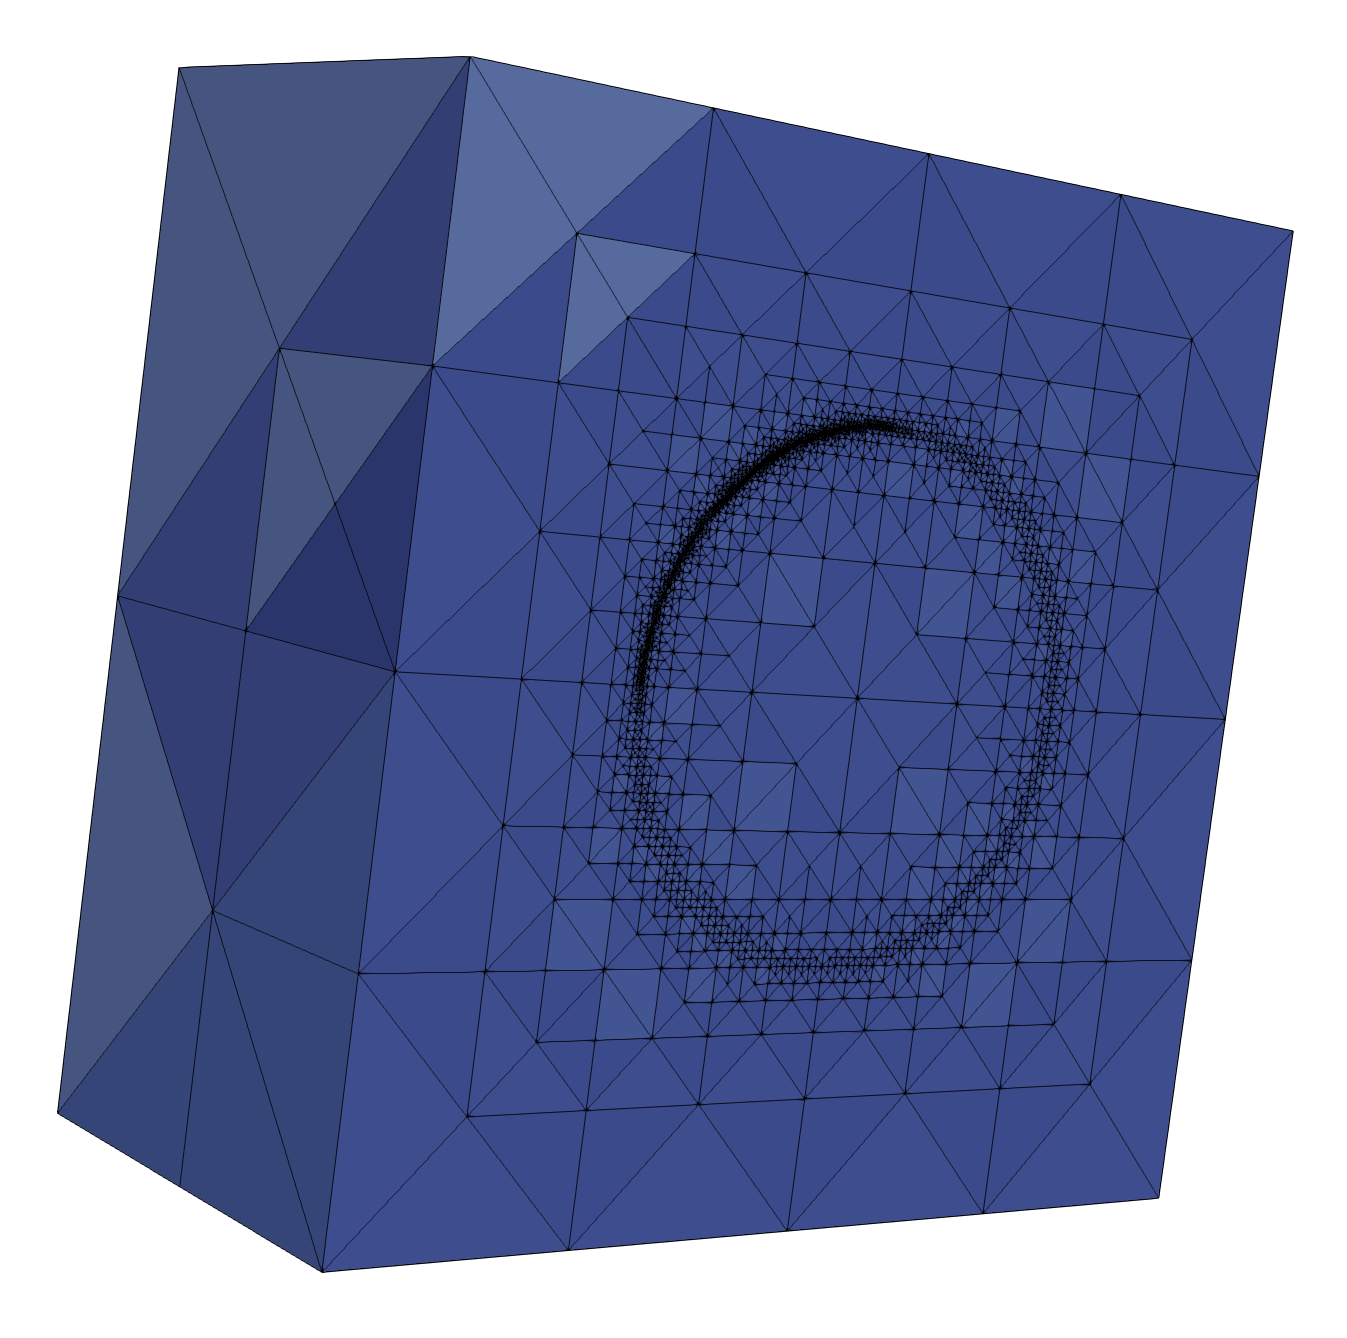
\includegraphics[width=0.40\linewidth]{figures/3d_sphere} 
	\caption{Result for sphere refinement pattern. Left: 2D. Right: 3D.}
	\label{fig:sphere}
\end{figure}

\section{Quality for recursive longest-edge}

\begin{figure}[htbp]
	\centering
	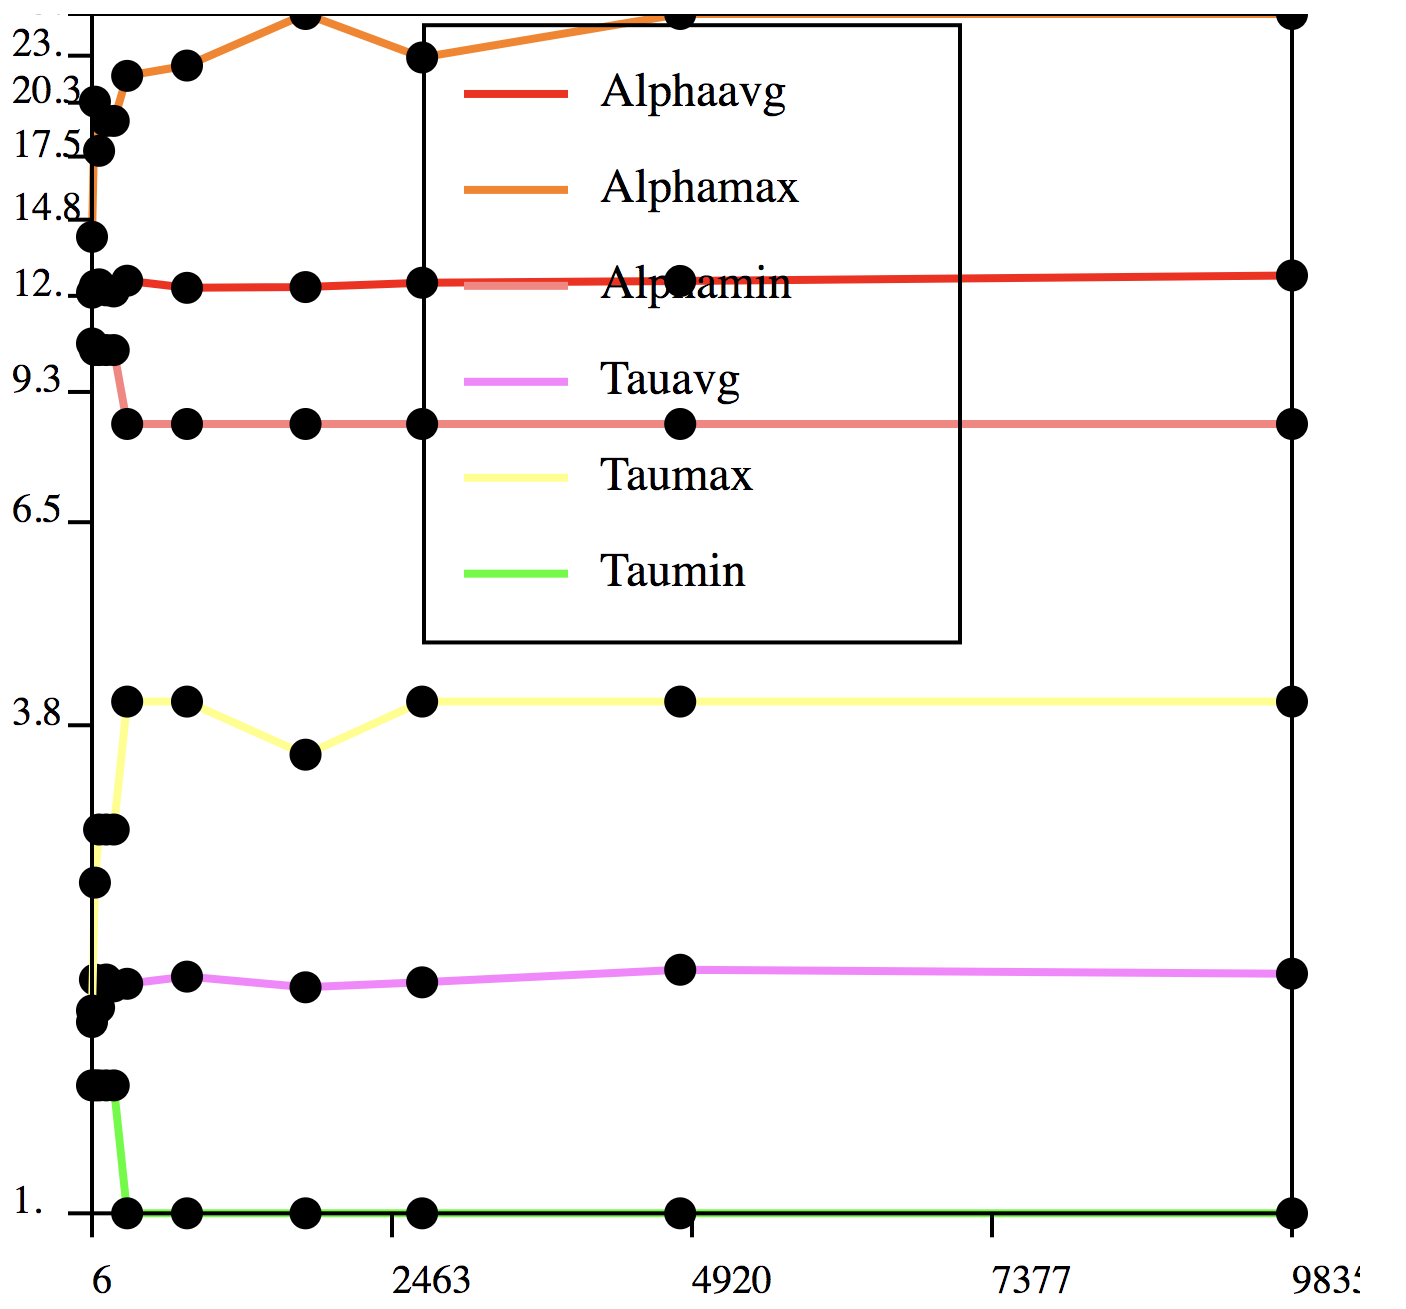
\includegraphics[width=0.48\linewidth]{figures/quality3} \hfill
	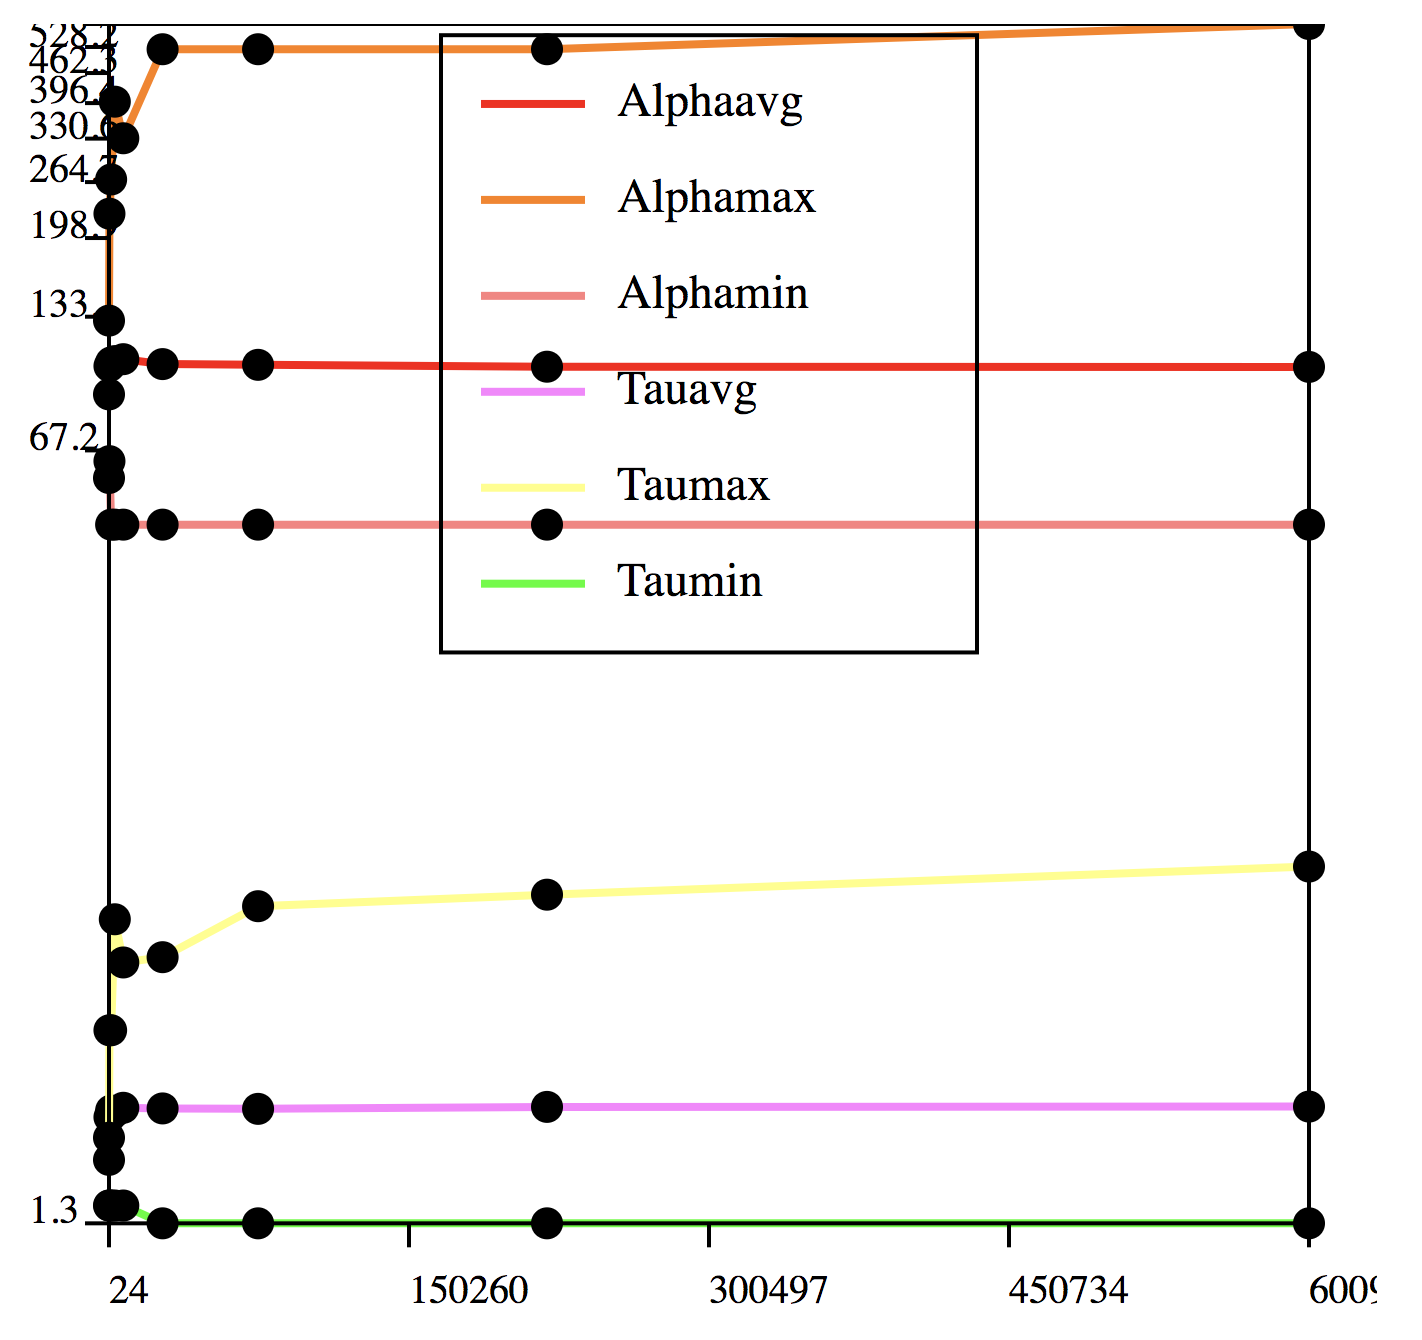
\includegraphics[width=0.48\linewidth]{figures/quality4} 
	\caption{Quality of the elements for several iterations of the adaptive refinement shown in Figure~\ref{fig:sphere}. The $x$ axis represent the total number of elements in the mesh. The $y$ axis the quality criterion (lower is better).
	 Left: 3D. Right: 4D.}
	\label{fig:quality}
\end{figure}

\begin{figure}[htbp]
	\centering
	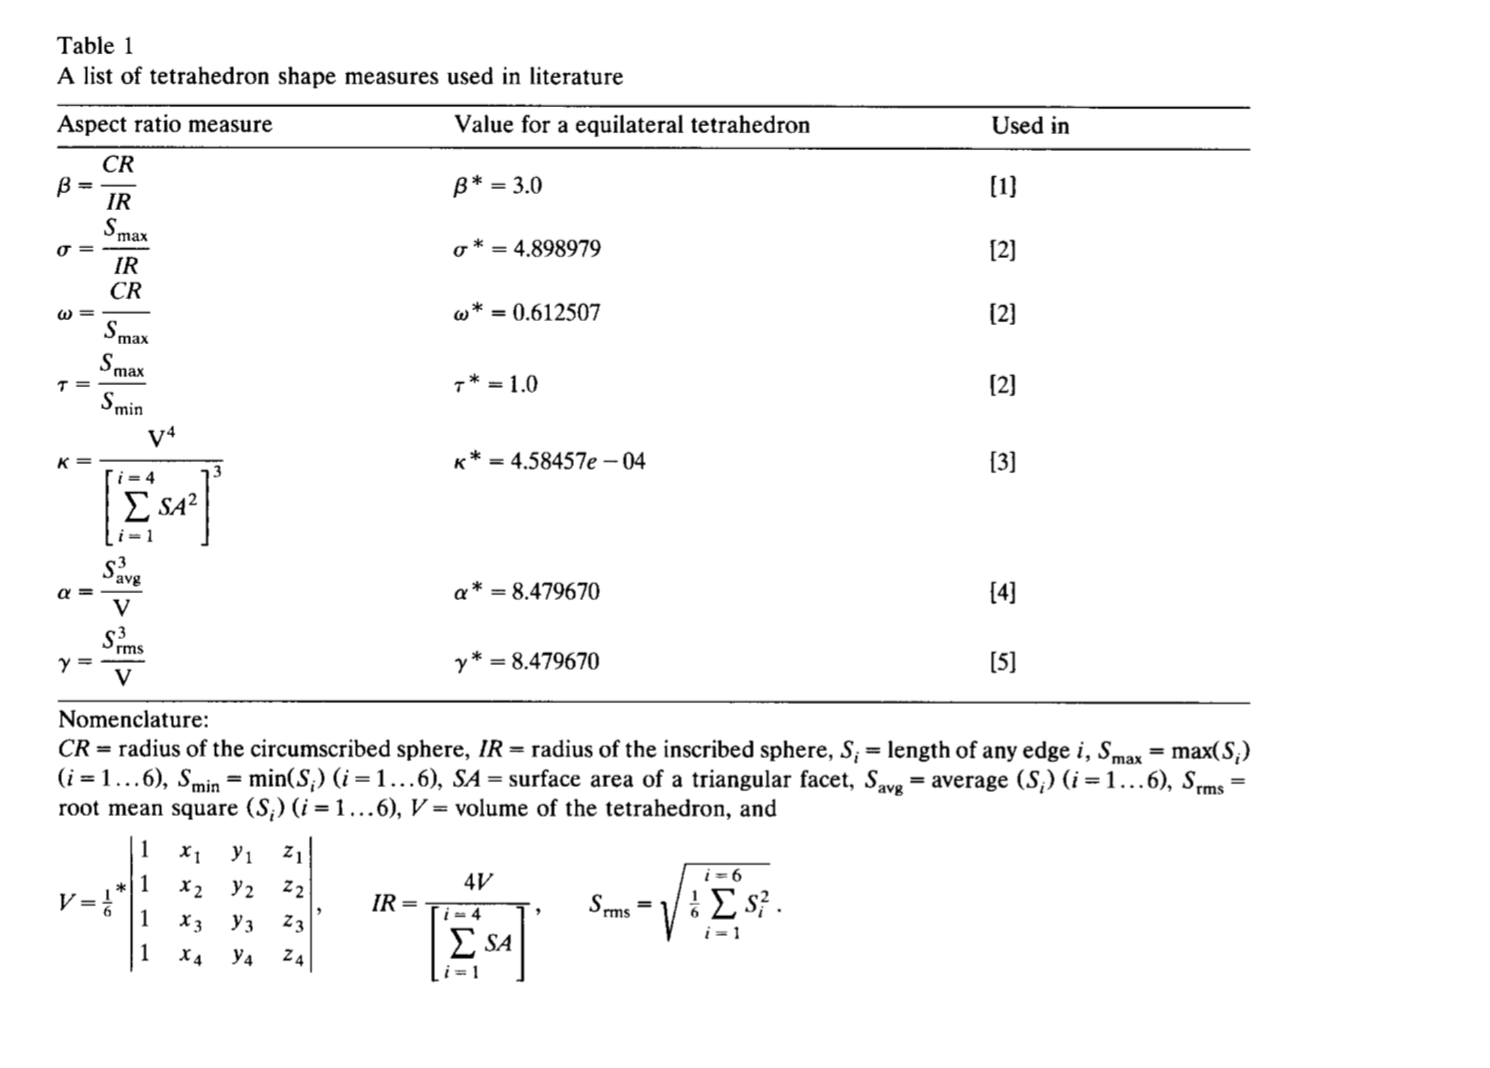
\includegraphics[width=0.8\linewidth]{figures/quality_metrics}
	\caption{Quality metics. We used ``Alpha'' and ``Tau''. }
	\label{fig:metrics}
\end{figure}



\clearpage

\section{Newest-vertex with longest edge for $D>2$}

Without a recurisve closure of the refined edge the overall element quality degrades very fast.

\begin{figure}[htbp]
	\centering
	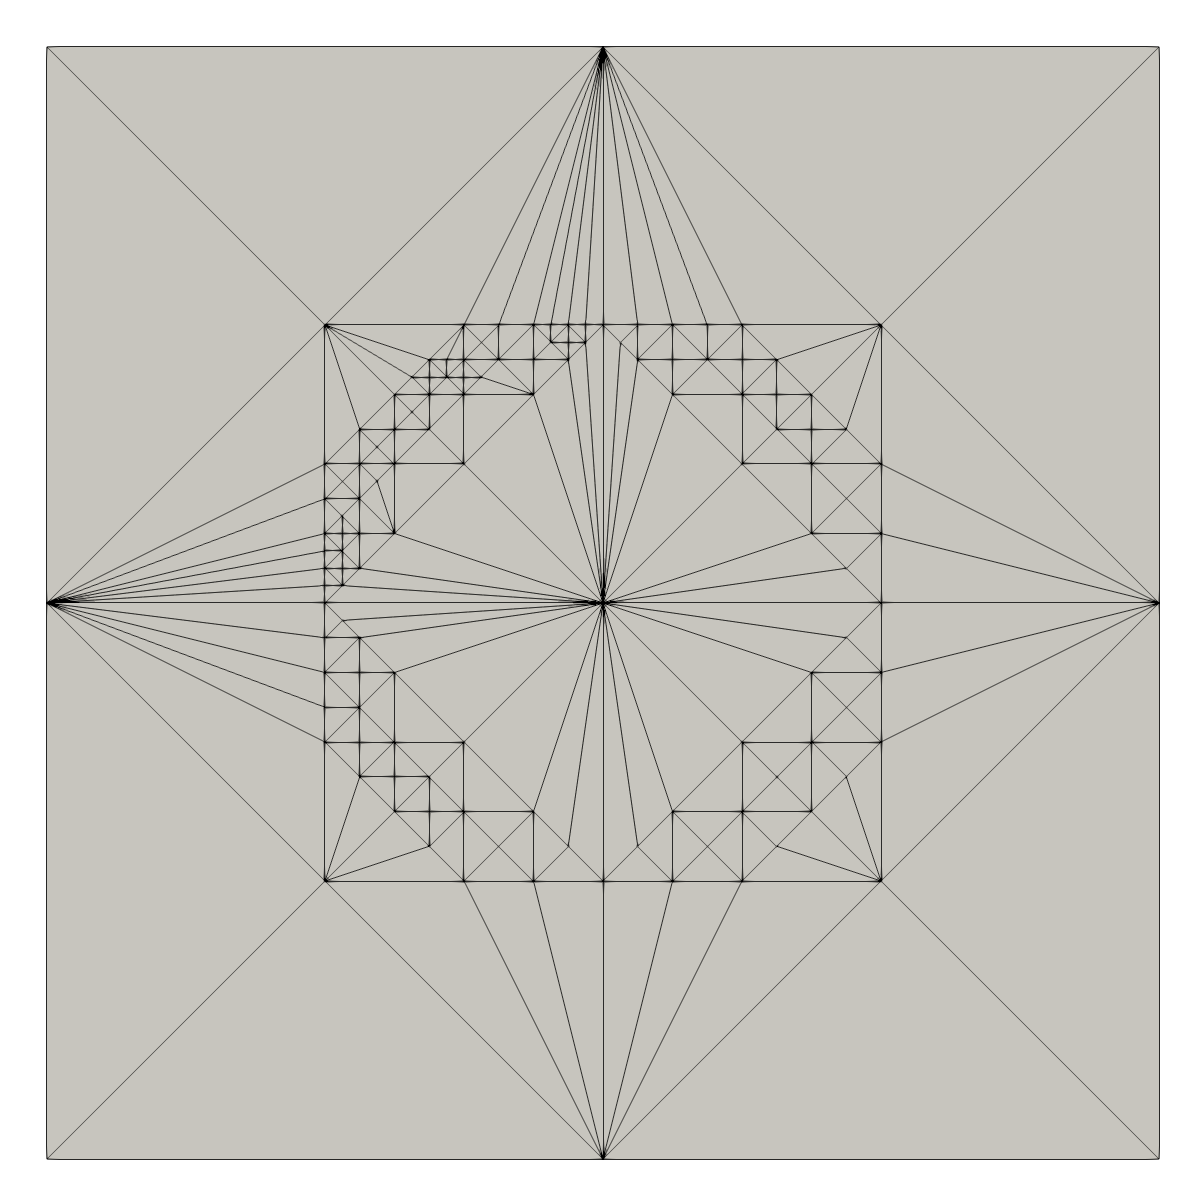
\includegraphics[width=0.48\linewidth]{figures/non-recursive} \hfill
	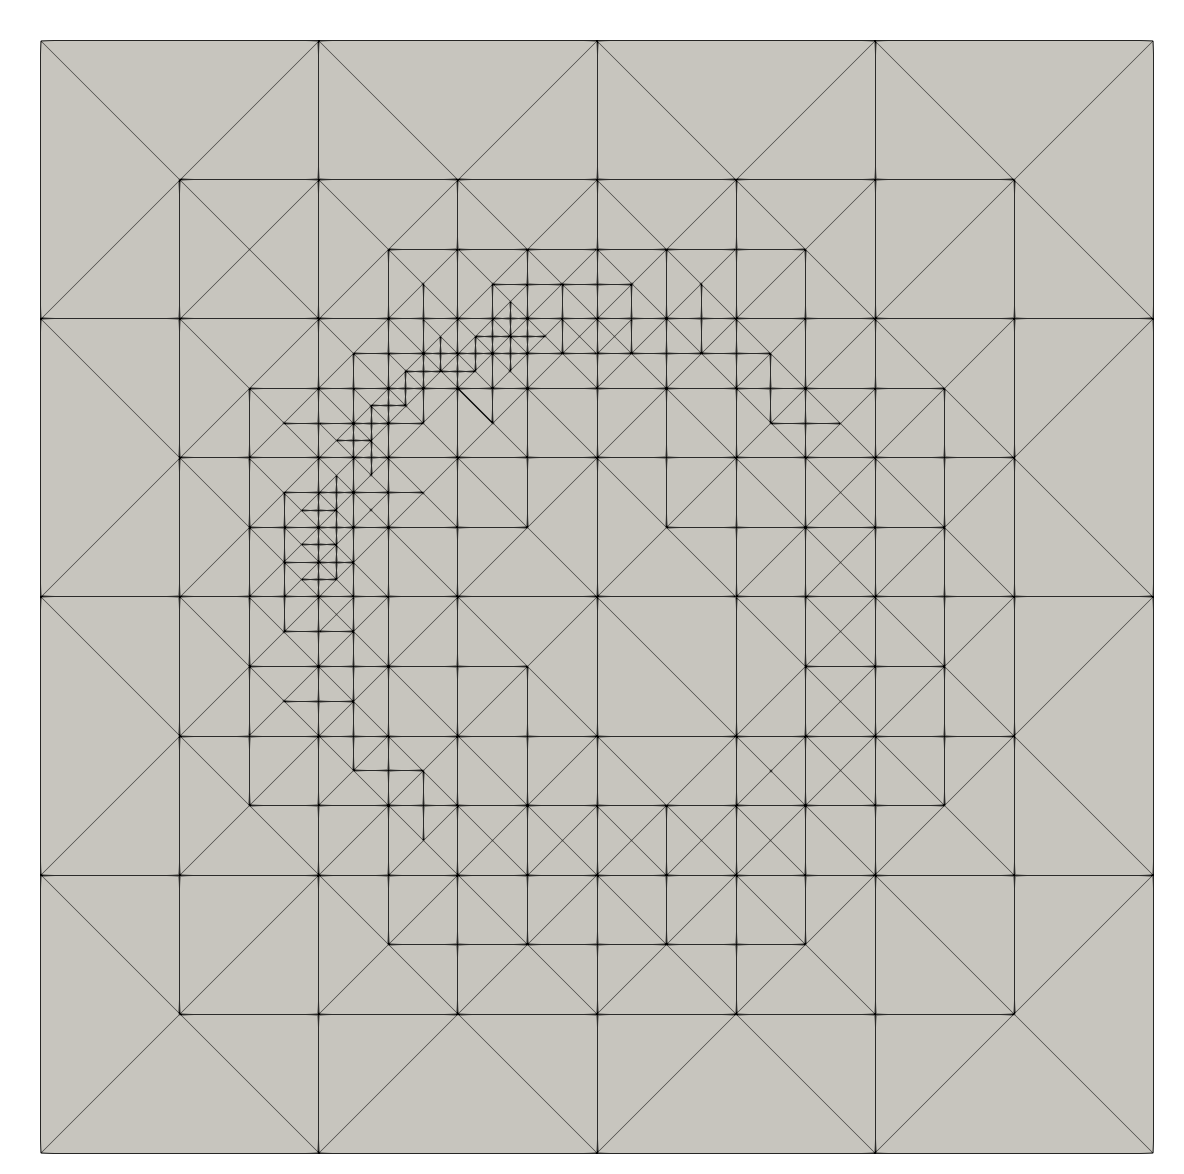
\includegraphics[width=0.48\linewidth]{figures/recursive}
	\caption{Non-recursive vs. recursive (3D).}
	\label{fig:metrics}
\end{figure}

\section{Quality of newest vertex with longest edge.}

While the longest-edge criterion is superior the hybrid approach (newest vertex + longest edge) 
stays in the same order of magnitude for the degrading element quality.

\begin{figure}[htbp]
	\centering
	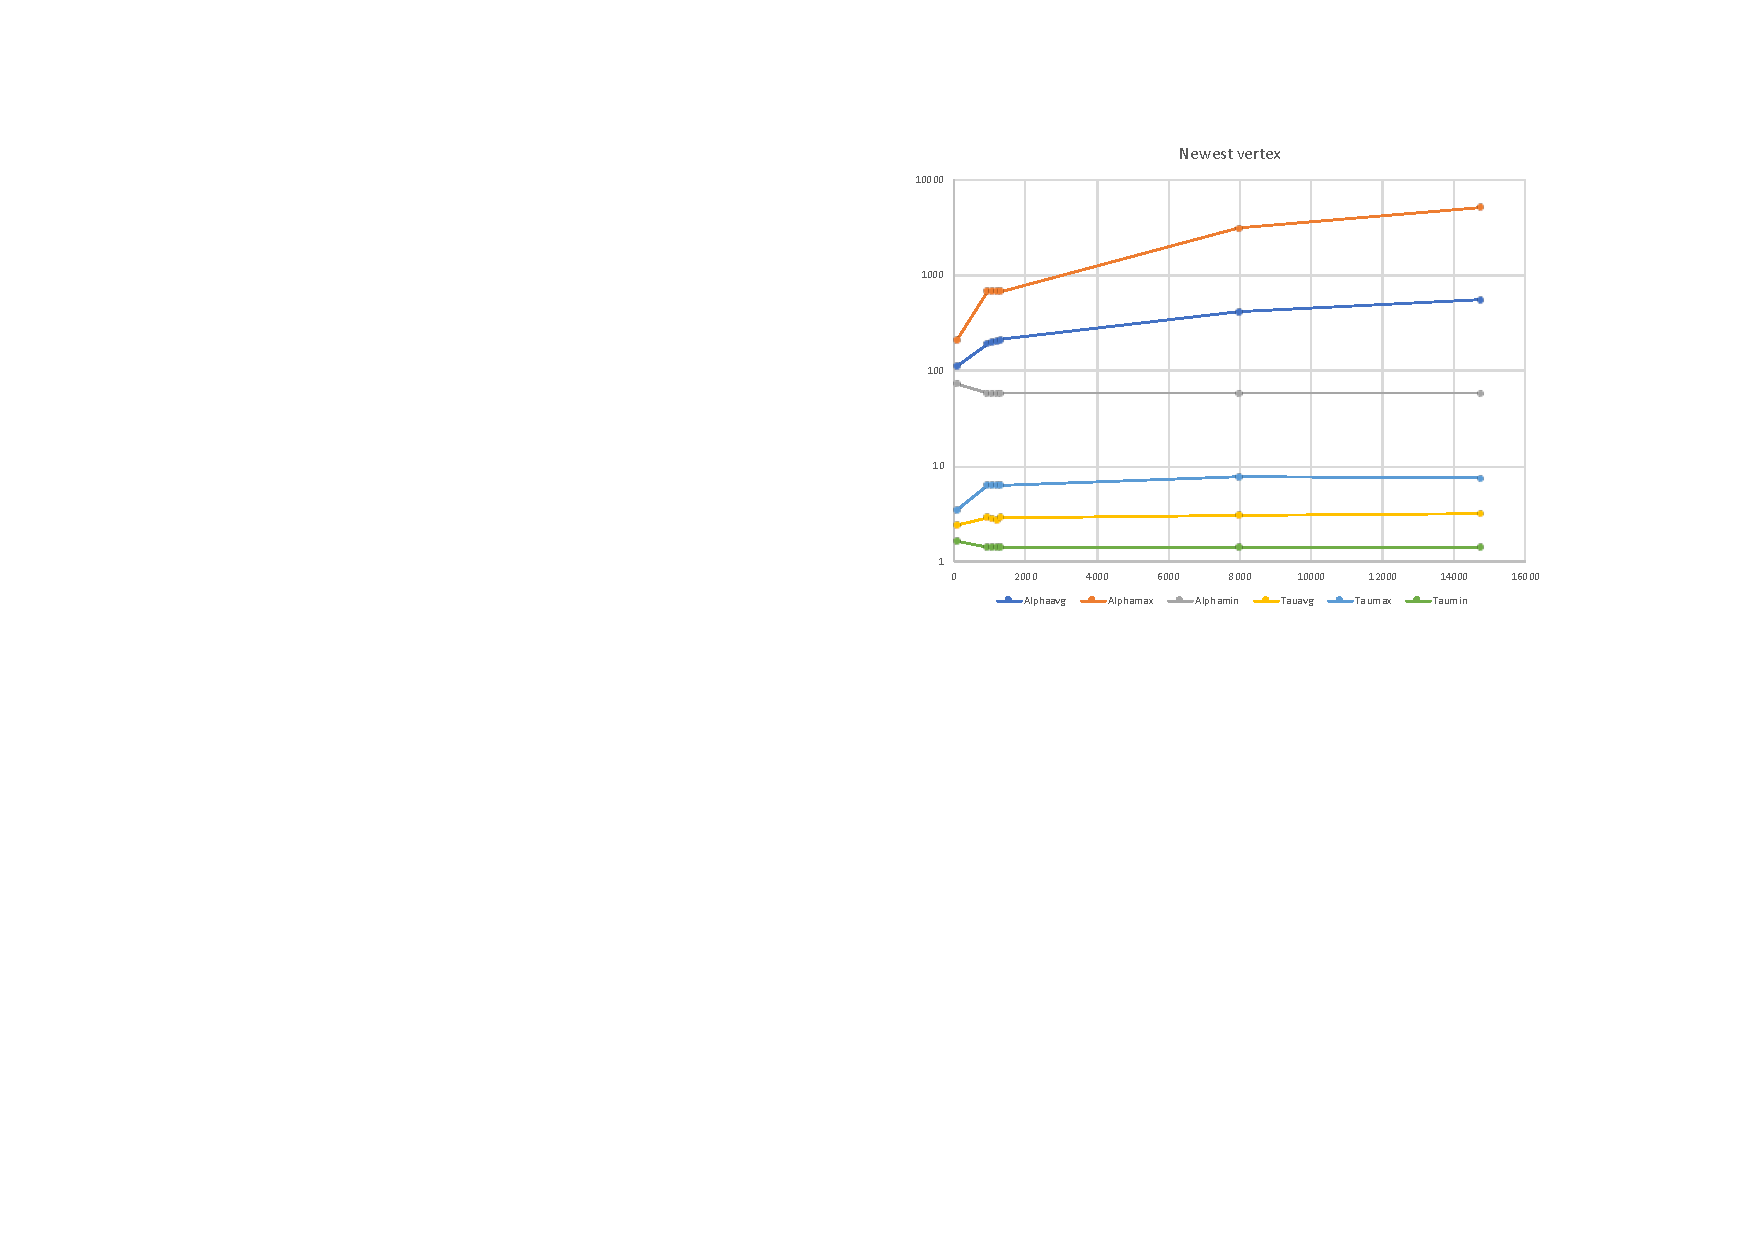
\includegraphics[width=0.48\linewidth]{figures/NewestVertex_Recursive} \hfill
	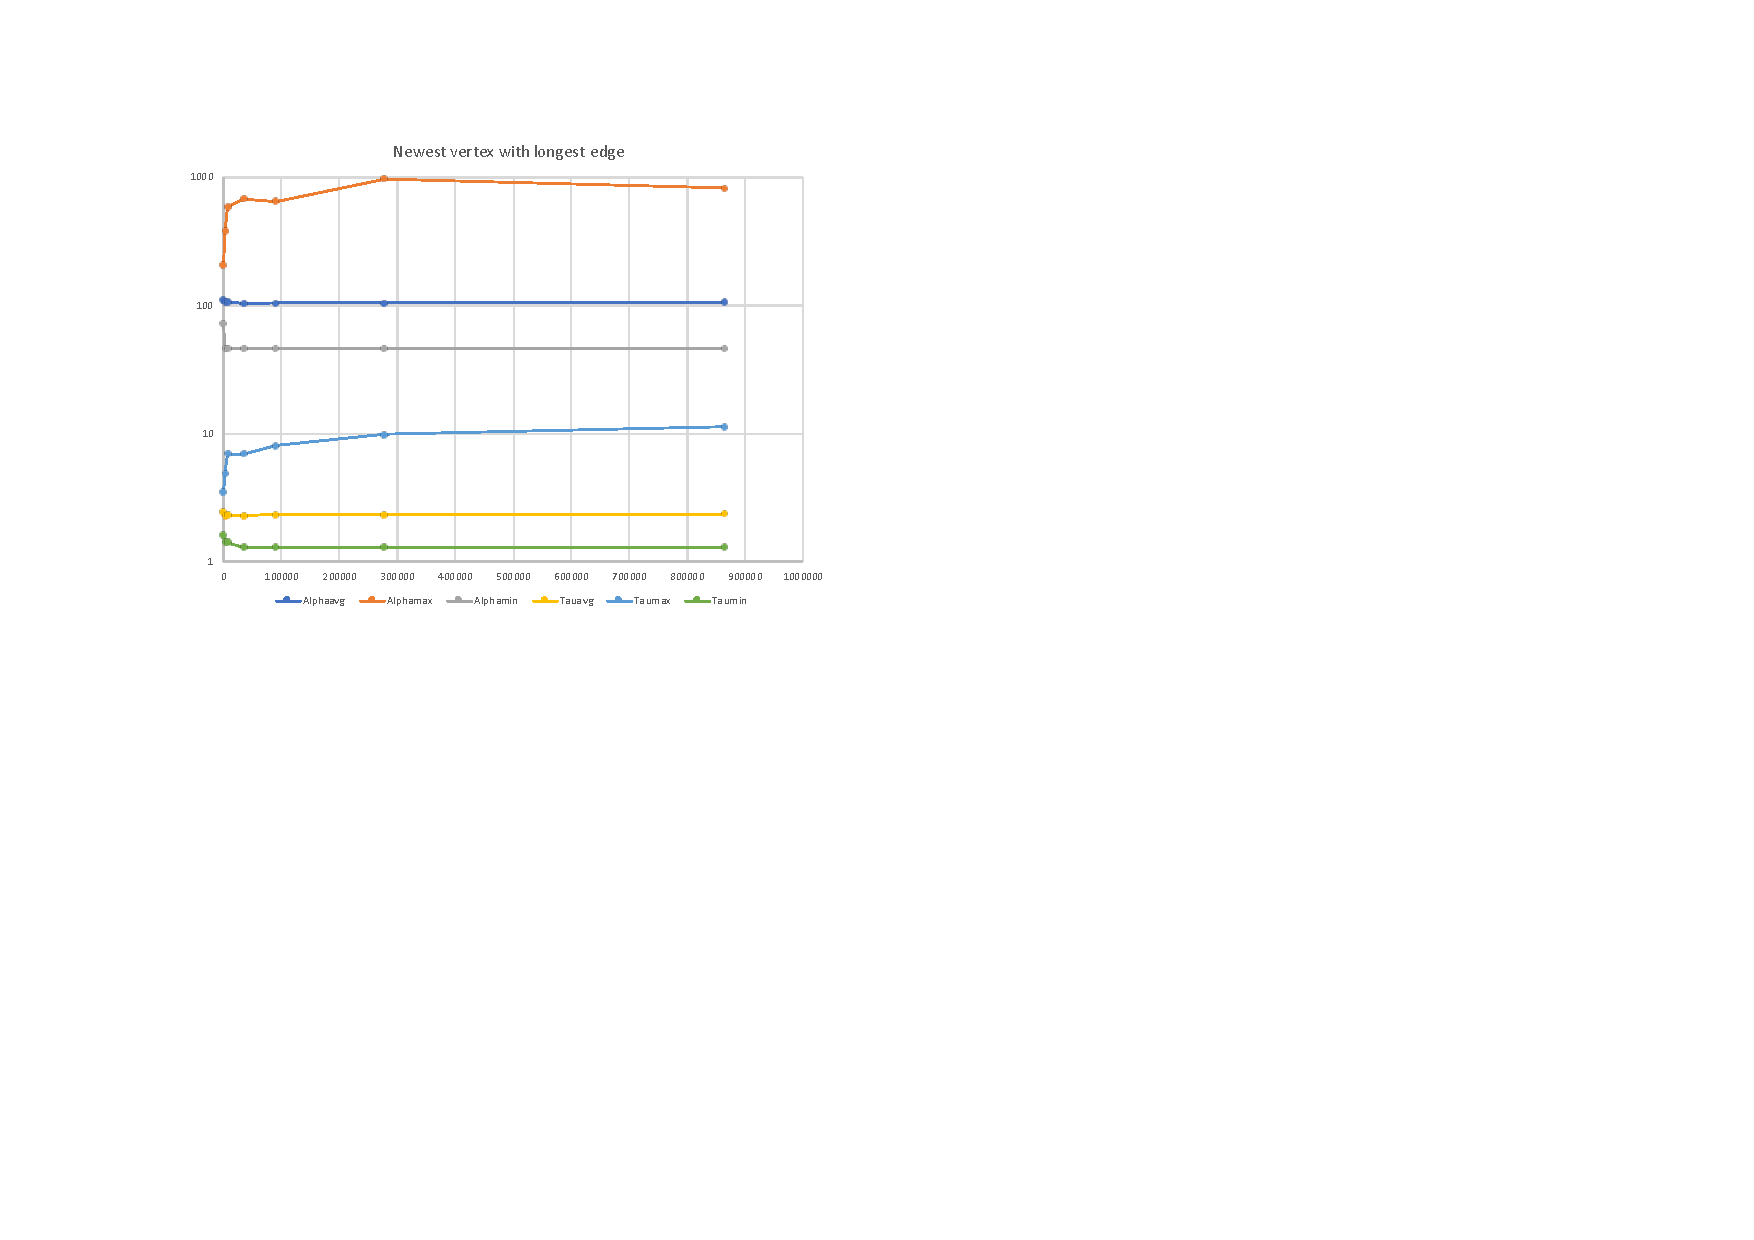
\includegraphics[width=0.48\linewidth]{figures/NewestVertex_and_LongestEdge_Recursive} 

	\caption{Quality of the elements for several iterations of the adaptive refinement shown in Figure~\ref{fig:sphere}. The $x$ axis represent the total number of elements in the 4D mesh. The $y$ axis the quality criterion (lower is better). The influence of longest edge shows on both the better quality and the larger number of elements generated.}
	\label{fig:quality}
\end{figure}


\section{Parallelization}

\begin{figure}[htbp]
	\centering
	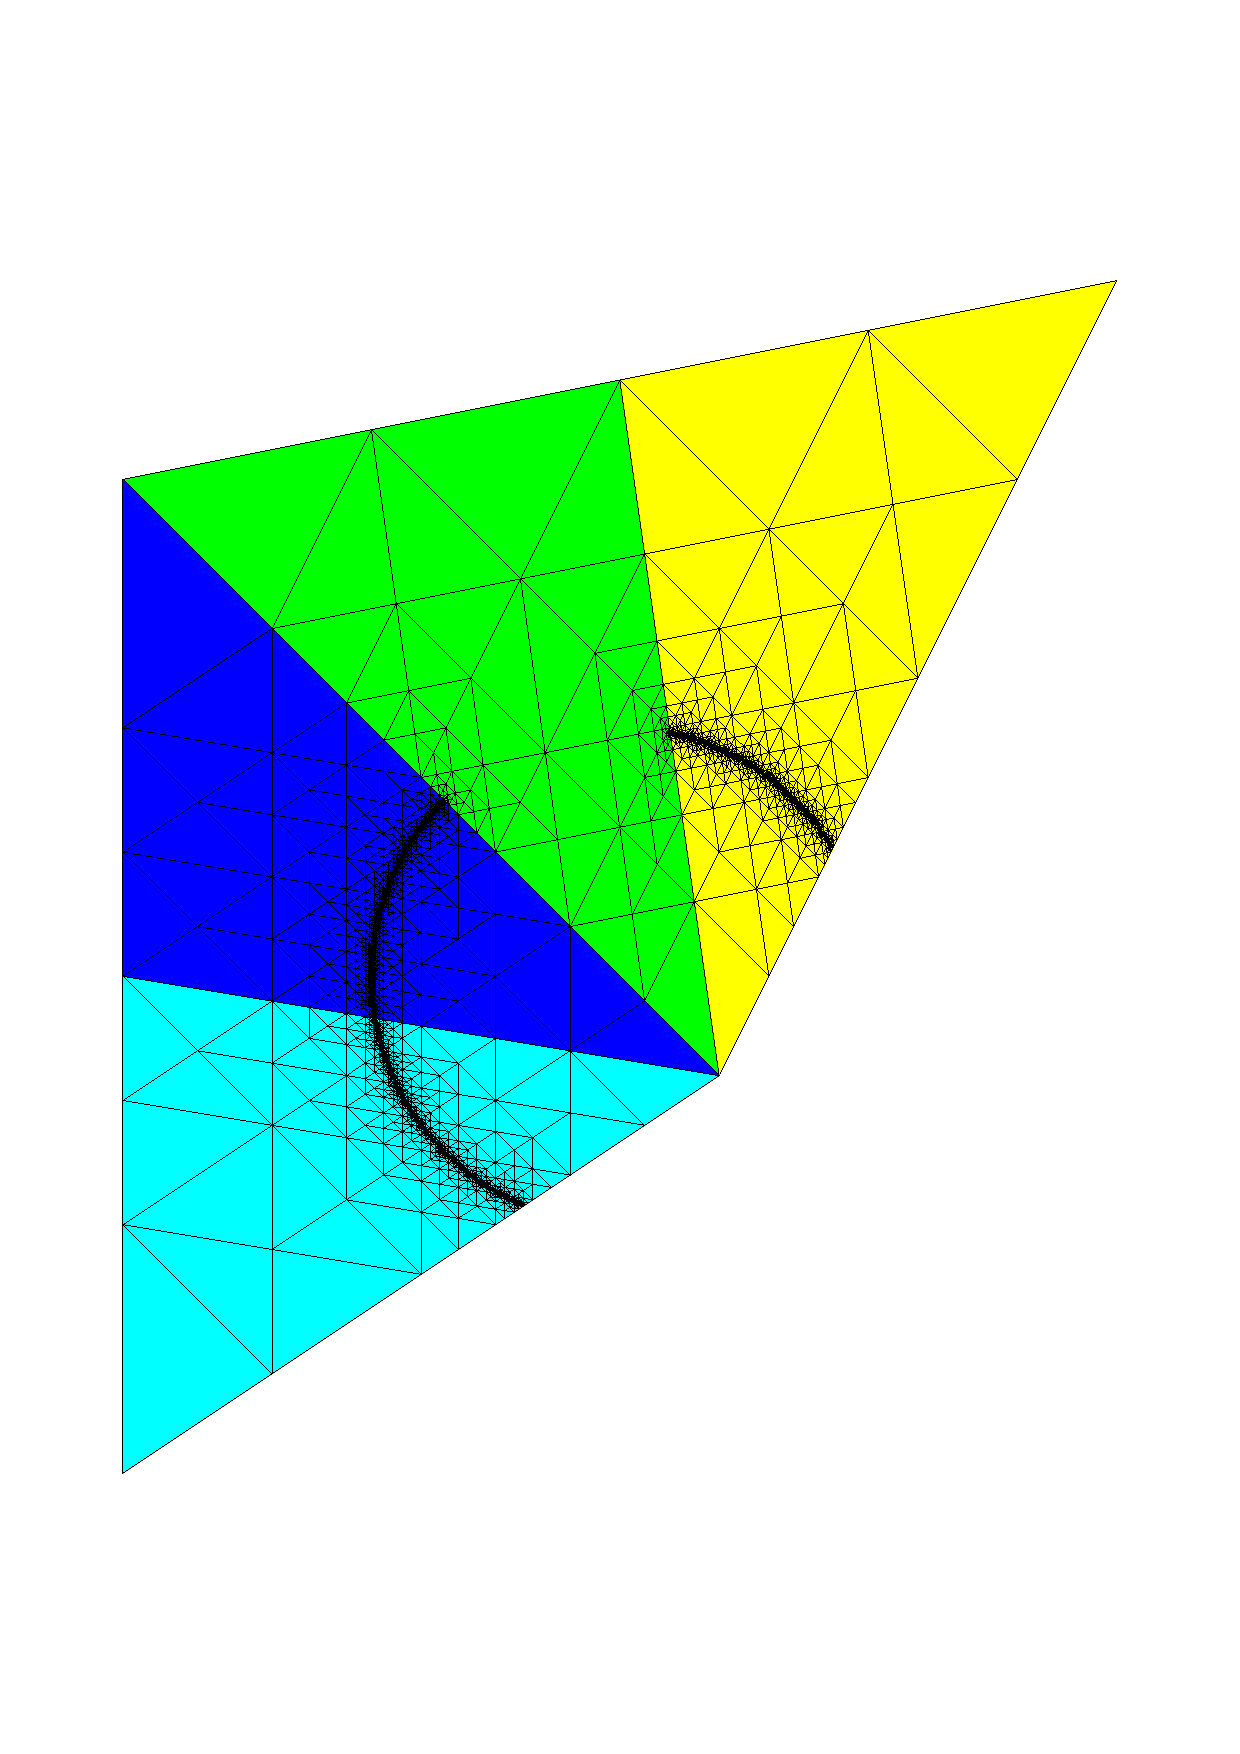
\includegraphics[width=0.8\linewidth]{figures/partitioning_with_one_part_without_refinement}
	\caption{Partitioning with one part without refinement.}
	\label{fig:metrics}
\end{figure}



\end{document}